\documentclass[tikz,border=5]{standalone}
\usetikzlibrary{shapes}
\tikzset{shape example/.style={
    color=black!50, draw, fill=blue!10,
    inner xsep=0.5cm, inner ysep=0.5cm,
    minimum height=3cm,
}}
\begin{document}
\Huge
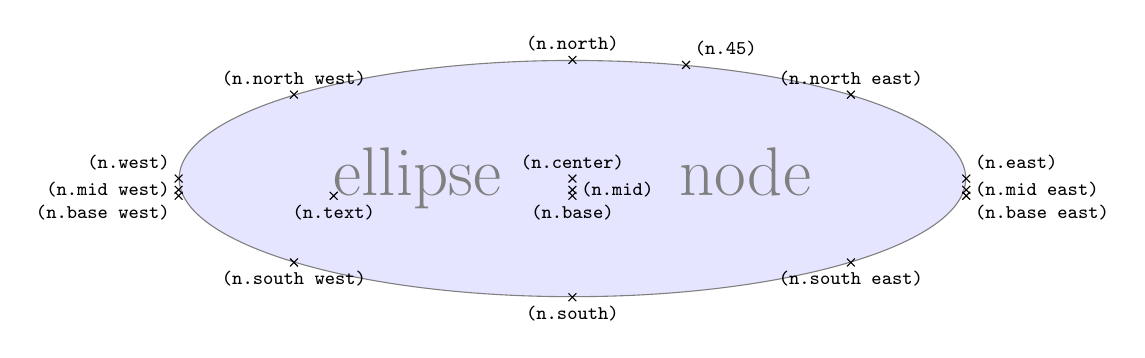
\begin{tikzpicture}[node distance = 1mm]
\node[name=n,shape=ellipse,shape example] {\Huge ellipse\hspace{2cm} node};
\foreach \anchor/\placement in
  {center/above, text/below, 45/above right,
     mid/right, mid east/right, mid west/left,
     base/below, base east/below right, base west/below left,
     north/above, south/below, east/above right, west/above left,
     north east/above, south east/below, south west/below, north west/above}
    \draw[shift=(n.\anchor)] plot[mark=x] coordinates{(0,0)}
      node[\placement,label distance = 0mm,inner sep=3pt] {\scriptsize\texttt{(n.\anchor)}};
\end{tikzpicture}
\end{document}
